%%%%%%%%%%%%%%%%%%%%%%%%%%%%%%%%%%%%%%%%%%%%%%%%%%%%%%%%%%%%%%%%%%%%%%%%
% This is the introduction chapter file.
%%%%%%%%%%%%%%%%%%%%%%%%%%%%%%%%%%%%%%%%%%%%%%%%%%%%%%%%%%%%%%%%%%%%%%%%
%
% Author:   René Widmer
%           Institute for Surgical Technology and Biomechanics ISTB
%           University of Bern
%           rene.widmer@istb.unibe.ch
%
% Date:     10/28/2009
%
%%%%%%%%%%%%%%%%%%%%%%%%%%%%%%%%%%%%%%%%%%%%%%%%%%%%%%%%%%%%%%%%%%%%%%%%

\chapter{Introduction}
\section{Motivation} 
\textcolor{red}{start with the clinical problem that you want to solve}

\textcolor{red}{why do we need navigation then, and why do we need yet another method?}
The goal of computer assisted surgeries is to reduce the time used to do the
surgery and to also improve the surgical result for the patient. In the case of
surgeries involving liver resections, navigation systems are rarely used because
they do not provide enough advantages compared to the additional time needed to
set them up. The accuracy of such navigation systems is affected by
deformations of the liver during the surgery \cite{clements2017deformation}.
Additionally for registration based methods is the registration error and the
time used to register the patient's anatomy to the preoperative 3D-model of the
liver. Supplementary these preoperative 3D-models are very expensive and time
consuming to generate. Therefore we aim to develop a new concept to navigate
during liver resections. This concept should not need a preoperative scan and would therefore
not need a registration. That way we would avoid the expensive and time
consuming preoperative 3D-model. 
\section{The Liver} 
\subsection{Liver Anatomy}
The human liver overlies the gallbladder, is located in the right upper quadrant of the abdomen and has
different functions. It produces biochemicals necessary for digestion,
synthesizes proteins and detoxifies various metabolites. A human liver wheighs
normally around 1.5 kg, is the heaviest internal organ and the largest gland
of the human body. Two large blood vessels are connected to the liver: the
portal vein and the hepatic vein. Both of them subdivide into small
capillaries called \textit{liver sinusoids} and then lead to the functional
units of the liver known as \textit{lobules}. To refer to the different parts of
the liver, it is subdivided into eight subsegments. Each segment has its own
vascular inflow and outflow.
\begin{figure}[H]
  \centering
 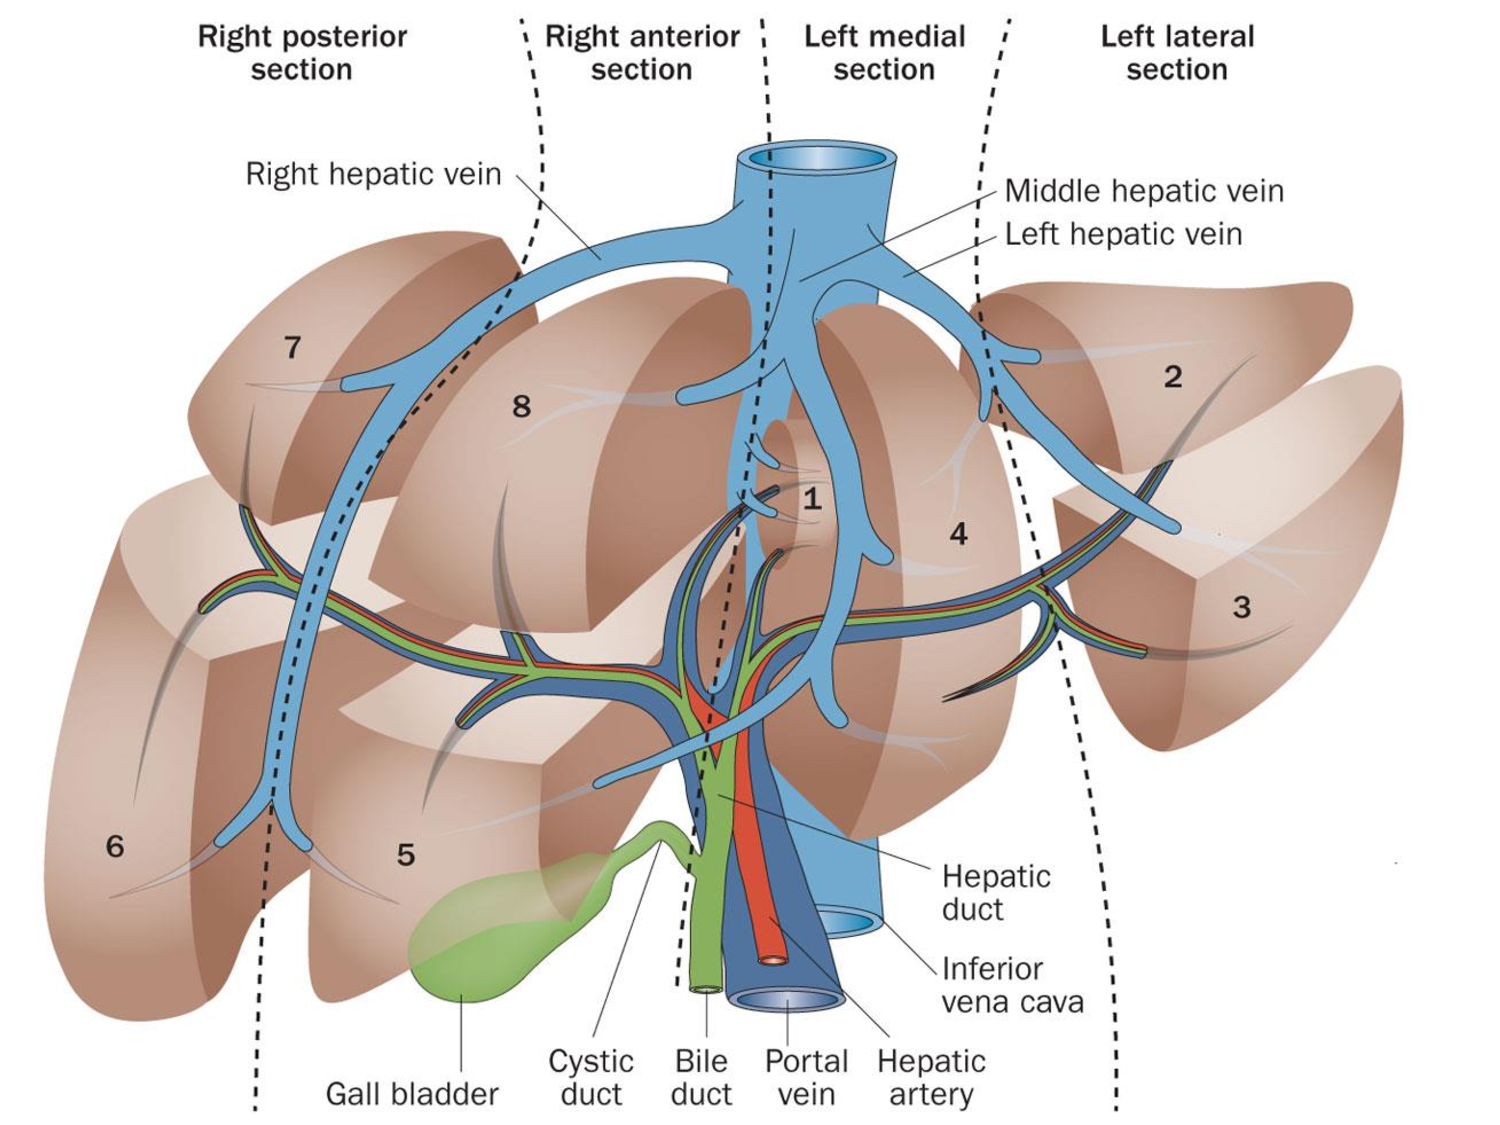
\includegraphics[width=\textwidth]{liverSegments}
  \caption{The liver and its eight Chouinaud segments. In red is the hepatic
    artery which transports blood from the heart a into the liver. In dark blue
    the portal vein, it transports blood from the gut into the liver. All the
    blood leavs the liver through the hepatic veins to the vena cava \cite{siriwardena2014management}.}
  \label{fig:liverSegments}
\end{figure}

\subsection{Liver Cancer}
\textcolor{green}{Liver metastatis are more common in US/Europe, in asia it's the other way around for example}

Liver cancer is cancer that starts in the liver. If the cancer has spread from
elsewhere to the liver, then it is known as liver metastasis. Liver metastasis
are about 20 times more common in the United States and in Europe than primary tumors. One of the reasons for that
is the rich blood supply of the liver which helps the tumors to grow
\cite{mcguire2016world}. In asia it's the other way round, more people suffer
from liver cancer than from liver metastases. Liver cancer patients often have chronic liver diseases
such as cirrhosis, problems of alcohol abuse, and viral hepatitis (B or C)
\cite{galun2015hepatocellular}. The gold standard to treat liver cancer are
surgical resections \cite{lencioni2012local}. The liver tissue can easily regrow, given that after resection there is
enough healthy tissue and blood supply preserved. Alternatively to resections
one can treat liver tumors by local ablation. Both variants treat the tumors
with a safety margin of 10 mm. This safety margin ensures that all tumor cells
are destroyed and to prevent further spread of cancer cells \cite{mahnken2009ct}.
\section{Liver Resections} 
\textcolor{green}{explain liver resections a bit more in detail, also what instruments are used and what to do with a blood vessel}
Hepatectomy is the surgical resection (removal of all or part) of the liver.
Liver resections are considered major surgeries and are done under general
anesthesia. If no other internal organs of the body are affected and the liver
is not cirrhotic, then 70\% to 80\% of the total liver volume can be removed in a
surgical resection. For patients with cirrhotic livers, not more than 50\% of
the total liver volume should be removed \cite{pianka2011liver}. Liver tissue is
cut using instruments like the BiClamp® vessel-sealing device (Figure \ref{fig:BiClampExplained}). Such devices can
simultaneously transect liver parenchyma and seal vessels with diameters smaller
than 7 mm \cite{zhao2017biclamp}. For larger vessels, resorbable clamps are used
to prevent undesired bloodflow out of the liver.
\begin{figure}[H]
  \centering
  \minipage{0.32\linewidth}
  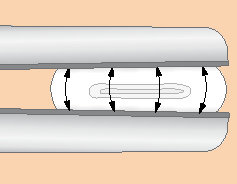
\includegraphics[width=\linewidth]{BiClamp1}
  \endminipage
  \hfill
  \minipage{0.32\linewidth}
  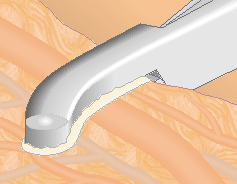
\includegraphics[width=\linewidth]{BiClamp2}
  \endminipage
  \hfill
  \minipage{0.32\linewidth}
  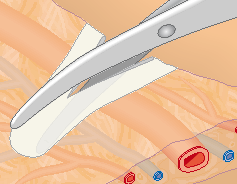
\includegraphics[width=\linewidth]{BiClamp3}
  \endminipage
  \hfill 
 \caption{A vessel sealing device is used to transect liver parenchyma and split
   blood vessels then seal them so that no blood is lost. From left to right:
   First, the vessel is pressed together and then the tissue coagulated using a bipolar
   electrosurgical current. In some cases this is done twice. Finally the tissue
   is separated mechanically at the center of the visible coagulation area \cite{biClampPdfWithImages}. }
  \label{fig:BiClampExplained}
\end{figure}

Most hepatectomies are done laparoscopicly. However for complicated
cases also open surgeries are done \cite{cherqui2000laparoscopic}. Two
resection techniques can be separated. Anatomical or parenchymal-sparing
resections (Figure \ref{fig:resectionsPlanning}). This work will concentrate on the latter technique. 
\begin{figure}[H]
  \centering
 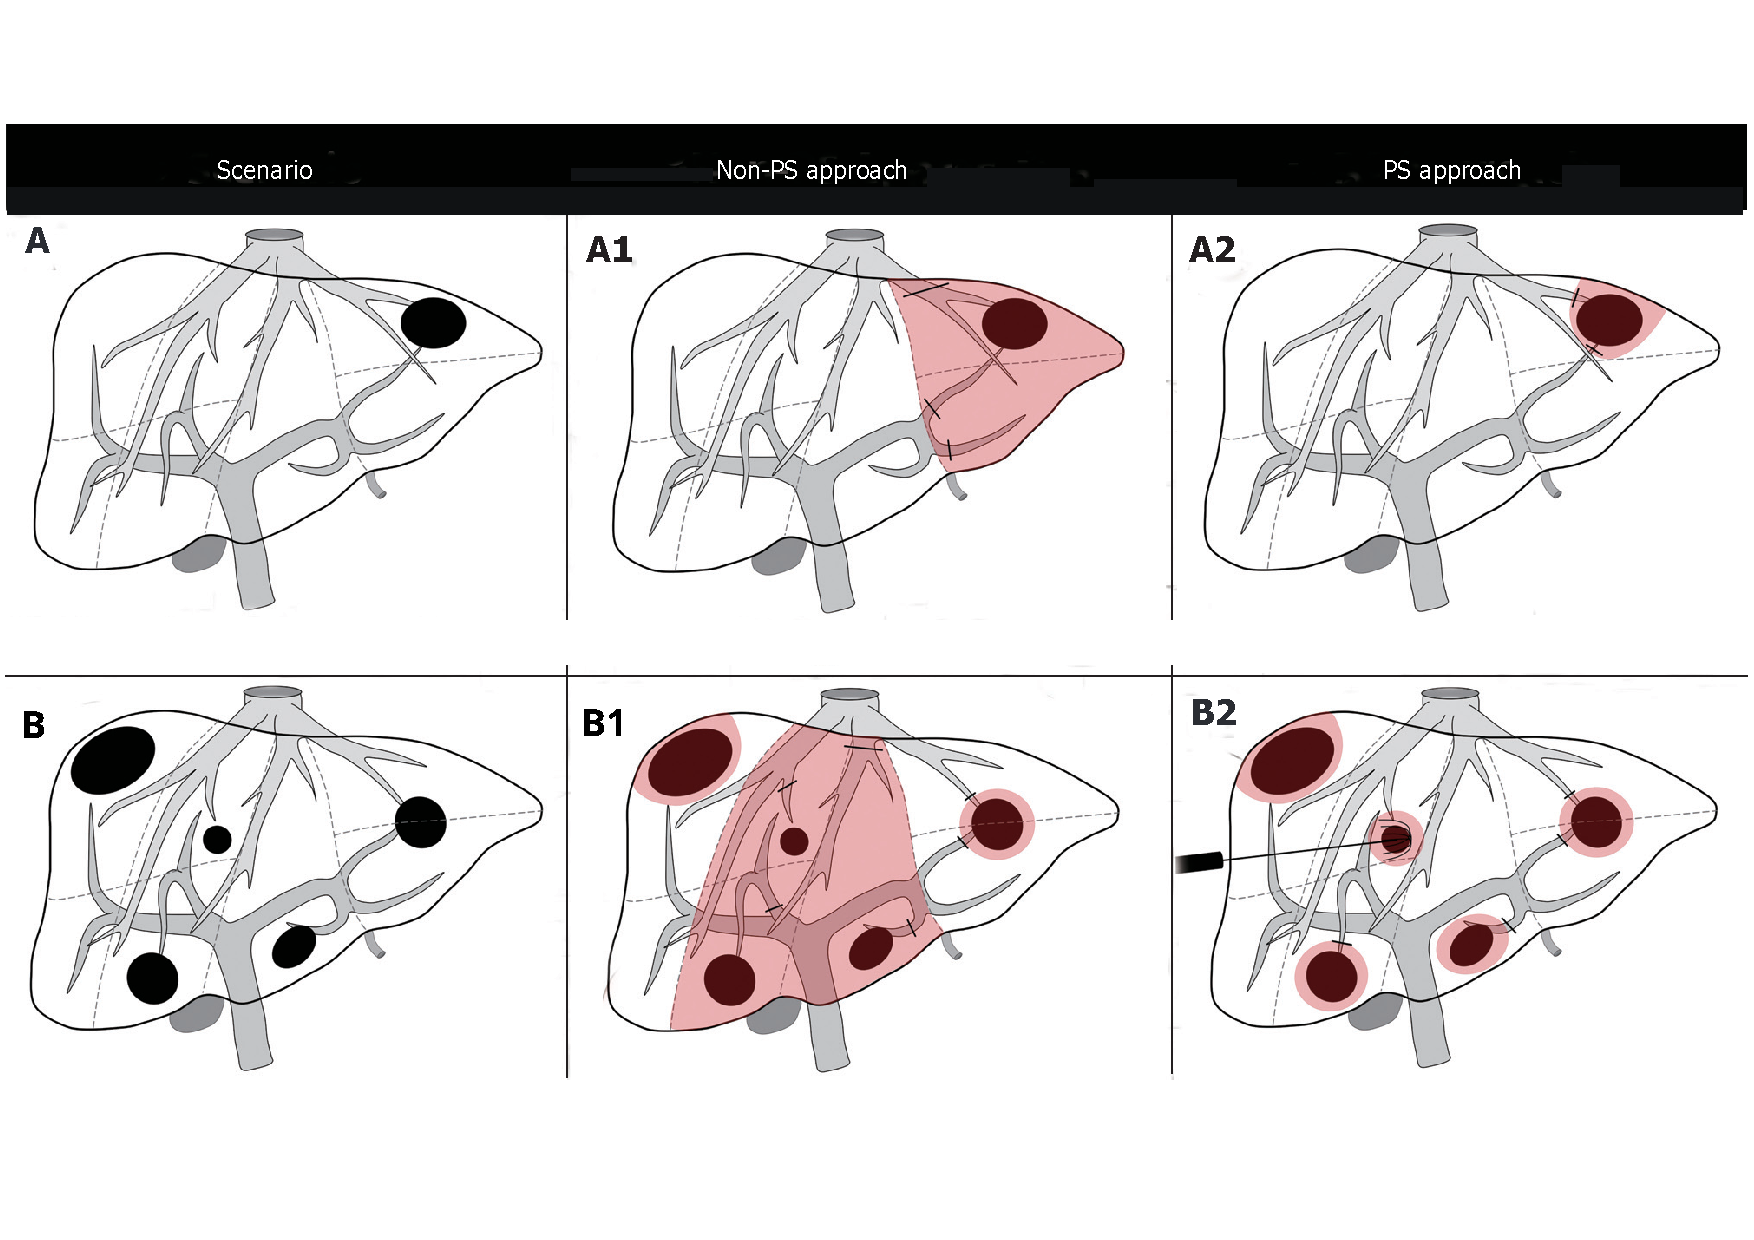
\includegraphics[width=\textwidth]{resectionsPlanning}
  \caption{Two different approaches to resect liver tumors in two different
    situations. The \textit{Scenario} column shows the situation of the
    patient's liver, the \textit{Non-PS approach} column shows how an anatomical
  resection plan would look like and the \textit{PS approach} column shows how a
parenchymal-sparing resection plan would look like \cite{alvarez2016parenchymal}.}
  \label{fig:resectionsPlanning}
\end{figure}


\subsection{Parenchymal-sparing liver surgeries}
Resection is the established gold-standard treatment of colorectal liver
metastases. The surgical treatment of colorectal liver metastases has changed with the expansion of the
parenchymal-sparing liver resection technique. This technique involves preserving healthy
functional liver parenchyma by performing a wide range of liver resections. In
order to perform the appropriate type of resection, the site and
relationships of the tumor with glissonian pedicles or hepatic veins have to be
known.
For that reason, it is obvious that only the heavy use of intraoperative liver
ultrasound makes it possible to perform parenchymal-sparing liver resections.
This can be also used with the laparoscopic approach. The method is backed by technical, oncological,
and pathological arguments.
This approach has multiple benefits: decreases postoperative mortality and
morbidity rates, while preserving the function of the liver. In turn, the risk
of liver dysfunction is reduced and the possibility of re-resection in case of
reccurence increases. Overall, parenchymal-sparing liver surgeries offer
similar survival results \cite{Ferrero2017}.

\cite{alvarez2016parenchymal}
\section{Objectives} 
The objectives of this Master's thesis are:
\begin{itemize}
  \item Implementation of the concept for an intraoperative 3D reconstrction
  technique of the liver from intraoperative ultrasound. 
  \item Implementation of the intraoperative resection planning.
\end{itemize}
This work focuses on open surgical procedures of liver hepatectomies and
especially parenchymal-sparing methods.


%Laparoscopic anatomical hepatectomy (LAH)

\endinput
%%% Local Variables:
%%% TeX-master: "MscThesis"
%%% End: